\documentclass{standalone}
\usepackage{tikz}
\usetikzlibrary{patterns, positioning}


\begin{document}
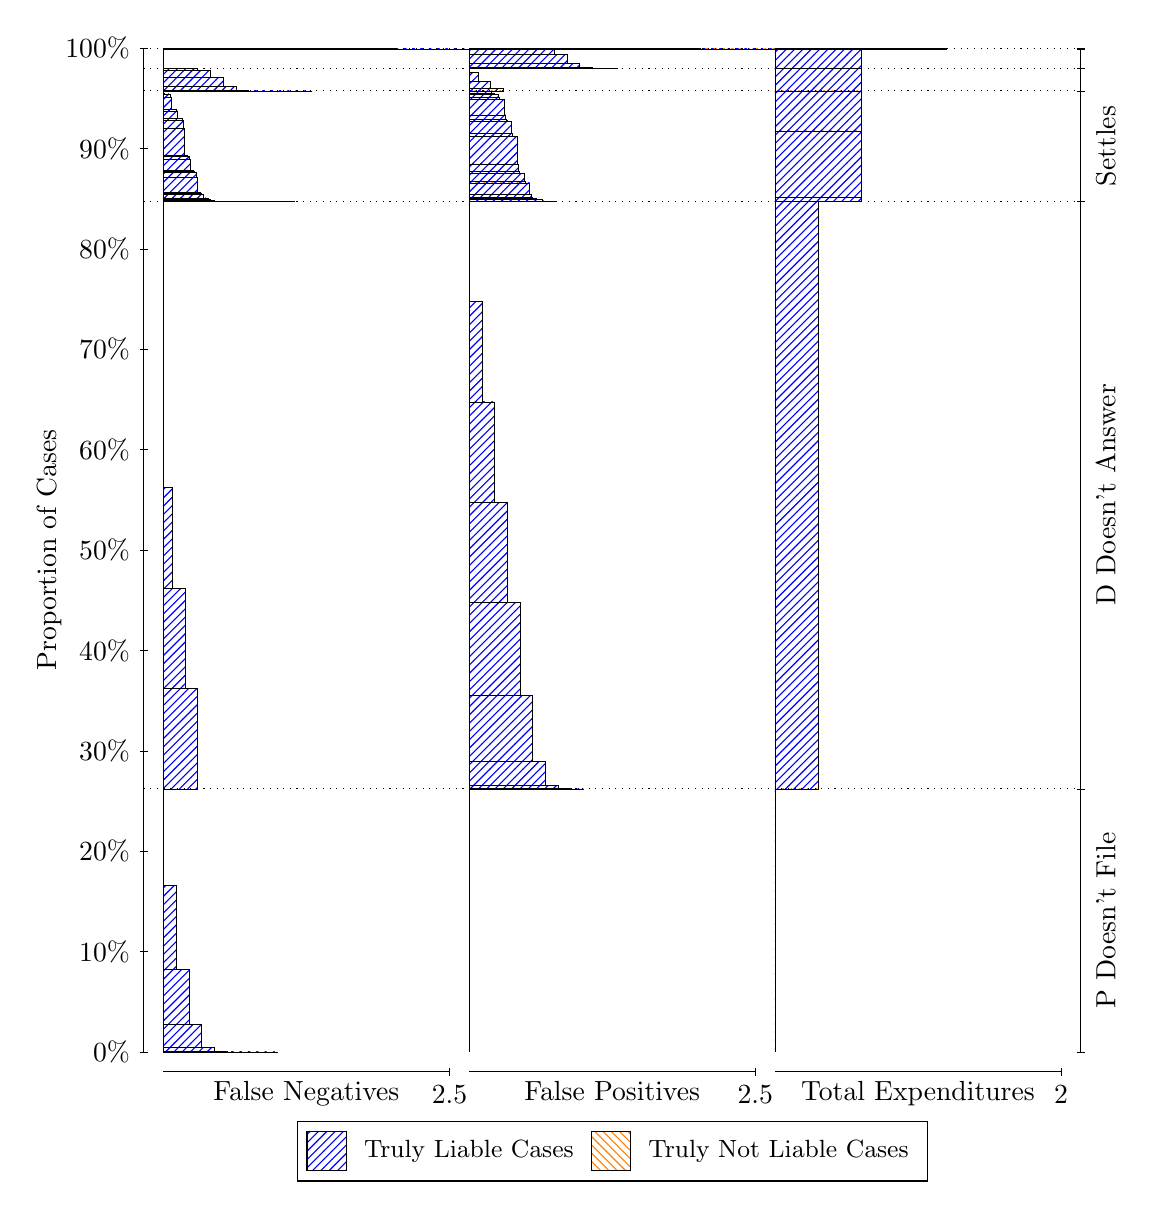
\begin{tikzpicture}
\draw[black, very thin] (1.5,1.75) -- (1.5,14.5);
\node[rotate=90, text=black, anchor=center] at (0.3, 8.125) {Proportion of Cases};
\draw[black, very thin] (1.45,1.75) -- (1.55,1.75);
\node[text=black, anchor=east] at (1.45, 1.75) {0\%};
\draw[black, very thin] (1.45,3.025) -- (1.55,3.025);
\node[text=black, anchor=east] at (1.45, 3.025) {10\%};
\draw[black, very thin] (1.45,4.3) -- (1.55,4.3);
\node[text=black, anchor=east] at (1.45, 4.3) {20\%};
\draw[black, very thin] (1.45,5.575) -- (1.55,5.575);
\node[text=black, anchor=east] at (1.45, 5.575) {30\%};
\draw[black, very thin] (1.45,6.85) -- (1.55,6.85);
\node[text=black, anchor=east] at (1.45, 6.85) {40\%};
\draw[black, very thin] (1.45,8.125) -- (1.55,8.125);
\node[text=black, anchor=east] at (1.45, 8.125) {50\%};
\draw[black, very thin] (1.45,9.4) -- (1.55,9.4);
\node[text=black, anchor=east] at (1.45, 9.4) {60\%};
\draw[black, very thin] (1.45,10.675) -- (1.55,10.675);
\node[text=black, anchor=east] at (1.45, 10.675) {70\%};
\draw[black, very thin] (1.45,11.95) -- (1.55,11.95);
\node[text=black, anchor=east] at (1.45, 11.95) {80\%};
\draw[black, very thin] (1.45,13.225) -- (1.55,13.225);
\node[text=black, anchor=east] at (1.45, 13.225) {90\%};
\draw[black, very thin] (1.45,14.5) -- (1.55,14.5);
\node[text=black, anchor=east] at (1.45, 14.5) {100\%};

\draw[black, very thin] (13.4,1.75) -- (13.4,14.5);
\draw[black, very thin] (13.35,1.75) -- (13.45,1.75);
\node[anchor=west] at (13.35, 1.75) {};
\draw[black, very thin] (13.35,5.0914) -- (13.45,5.0914);
\node[anchor=west] at (13.35, 5.0914) {};
\draw[black, very thin] (13.35,12.555) -- (13.45,12.555);
\node[anchor=west] at (13.35, 12.555) {};
\draw[black, very thin] (13.35,13.957) -- (13.45,13.957);
\node[anchor=west] at (13.35, 13.957) {};
\draw[black, very thin] (13.35,14.245) -- (13.45,14.245);
\node[anchor=west] at (13.35, 14.245) {};
\draw[black, very thin] (13.35,14.489) -- (13.45,14.489);
\node[anchor=west] at (13.35, 14.489) {};
\draw[black, very thin] (13.35,14.5) -- (13.45,14.5);
\node[anchor=west] at (13.35, 14.5) {};

\draw[black, very thin, pattern color=blue, pattern=north east lines] (1.75,1.75) rectangle (3.2033,1.75);
\draw[black, very thin, pattern color=blue, pattern=north east lines] (1.75,1.75) rectangle (3.0419,1.75);
\draw[black, very thin, pattern color=blue, pattern=north east lines] (1.75,1.75) rectangle (2.8804,1.75);
\draw[black, very thin, pattern color=blue, pattern=north east lines] (1.75,1.75) rectangle (2.7189,1.7502);
\draw[black, very thin, pattern color=blue, pattern=north east lines] (1.75,1.7502) rectangle (2.5574,1.7554);
\draw[black, very thin, pattern color=blue, pattern=north east lines] (1.75,1.7554) rectangle (2.3959,1.8131);
\draw[black, very thin, pattern color=blue, pattern=north east lines] (1.75,1.8131) rectangle (2.2344,2.0967);
\draw[black, very thin, pattern color=blue, pattern=north east lines] (1.75,2.0967) rectangle (2.073,2.8013);
\draw[black, very thin, pattern color=blue, pattern=north east lines] (1.75,2.8013) rectangle (1.9115,3.8676);
\draw[black, very thin, pattern color=orange, pattern=north west lines] (1.75,3.8676) rectangle (1.75,3.8676);
\draw[black, very thin, pattern color=blue, pattern=north east lines] (1.75,3.8676) rectangle (1.75,5.0914);
\draw[black, very thin, pattern color=blue, pattern=north east lines] (1.75,5.0914) rectangle (2.186,6.3664);
\draw[black, very thin, pattern color=blue, pattern=north east lines] (1.75,6.3664) rectangle (2.0245,7.6414);
\draw[black, very thin, pattern color=blue, pattern=north east lines] (1.75,7.6414) rectangle (1.863,8.9161);
\draw[black, very thin, pattern color=orange, pattern=north west lines] (1.75,8.9161) rectangle (1.75,8.9161);
\draw[black, very thin, pattern color=blue, pattern=north east lines] (1.75,8.9161) rectangle (1.75,12.555);
\draw[black, very thin, pattern color=blue, pattern=north east lines] (1.75,12.555) rectangle (3.4213,12.555);
\draw[black, very thin, pattern color=blue, pattern=north east lines] (1.75,12.555) rectangle (3.3487,12.555);
\draw[black, very thin, pattern color=blue, pattern=north east lines] (1.75,12.555) rectangle (3.276,12.555);
\draw[black, very thin, pattern color=blue, pattern=north east lines] (1.75,12.555) rectangle (3.2599,12.555);
\draw[black, very thin, pattern color=blue, pattern=north east lines] (1.75,12.555) rectangle (3.2033,12.555);
\draw[black, very thin, pattern color=blue, pattern=north east lines] (1.75,12.555) rectangle (3.1872,12.555);
\draw[black, very thin, pattern color=blue, pattern=north east lines] (1.75,12.555) rectangle (3.1307,12.555);
\draw[black, very thin, pattern color=blue, pattern=north east lines] (1.75,12.555) rectangle (3.1145,12.555);
\draw[black, very thin, pattern color=blue, pattern=north east lines] (1.75,12.555) rectangle (3.0984,12.555);
\draw[black, very thin, pattern color=blue, pattern=north east lines] (1.75,12.555) rectangle (3.058,12.555);
\draw[black, very thin, pattern color=blue, pattern=north east lines] (1.75,12.555) rectangle (3.0419,12.555);
\draw[black, very thin, pattern color=blue, pattern=north east lines] (1.75,12.555) rectangle (3.0257,12.555);
\draw[black, very thin, pattern color=blue, pattern=north east lines] (1.75,12.555) rectangle (2.9853,12.555);
\draw[black, very thin, pattern color=blue, pattern=north east lines] (1.75,12.555) rectangle (2.9692,12.555);
\draw[black, very thin, pattern color=blue, pattern=north east lines] (1.75,12.555) rectangle (2.953,12.555);
\draw[black, very thin, pattern color=blue, pattern=north east lines] (1.75,12.555) rectangle (2.9369,12.555);
\draw[black, very thin, pattern color=blue, pattern=north east lines] (1.75,12.555) rectangle (2.8965,12.555);
\draw[black, very thin, pattern color=blue, pattern=north east lines] (1.75,12.555) rectangle (2.8804,12.555);
\draw[black, very thin, pattern color=blue, pattern=north east lines] (1.75,12.555) rectangle (2.8642,12.555);
\draw[black, very thin, pattern color=blue, pattern=north east lines] (1.75,12.555) rectangle (2.8239,12.555);
\draw[black, very thin, pattern color=blue, pattern=north east lines] (1.75,12.555) rectangle (2.8077,12.555);
\draw[black, very thin, pattern color=blue, pattern=north east lines] (1.75,12.555) rectangle (2.7916,12.555);
\draw[black, very thin, pattern color=blue, pattern=north east lines] (1.75,12.555) rectangle (2.7754,12.555);
\draw[black, very thin, pattern color=blue, pattern=north east lines] (1.75,12.555) rectangle (2.735,12.555);
\draw[black, very thin, pattern color=blue, pattern=north east lines] (1.75,12.555) rectangle (2.7189,12.555);
\draw[black, very thin, pattern color=blue, pattern=north east lines] (1.75,12.555) rectangle (2.7027,12.555);
\draw[black, very thin, pattern color=blue, pattern=north east lines] (1.75,12.555) rectangle (2.6624,12.555);
\draw[black, very thin, pattern color=blue, pattern=north east lines] (1.75,12.555) rectangle (2.6462,12.555);
\draw[black, very thin, pattern color=blue, pattern=north east lines] (1.75,12.555) rectangle (2.6301,12.555);
\draw[black, very thin, pattern color=blue, pattern=north east lines] (1.75,12.555) rectangle (2.6139,12.555);
\draw[black, very thin, pattern color=blue, pattern=north east lines] (1.75,12.555) rectangle (2.5736,12.555);
\draw[black, very thin, pattern color=blue, pattern=north east lines] (1.75,12.555) rectangle (2.5574,12.555);
\draw[black, very thin, pattern color=blue, pattern=north east lines] (1.75,12.555) rectangle (2.5413,12.555);
\draw[black, very thin, pattern color=blue, pattern=north east lines] (1.75,12.555) rectangle (2.5009,12.556);
\draw[black, very thin, pattern color=blue, pattern=north east lines] (1.75,12.556) rectangle (2.4847,12.556);
\draw[black, very thin, pattern color=blue, pattern=north east lines] (1.75,12.556) rectangle (2.4686,12.556);
\draw[black, very thin, pattern color=blue, pattern=north east lines] (1.75,12.556) rectangle (2.4524,12.557);
\draw[black, very thin, pattern color=blue, pattern=north east lines] (1.75,12.557) rectangle (2.4121,12.559);
\draw[black, very thin, pattern color=blue, pattern=north east lines] (1.75,12.559) rectangle (2.3959,12.561);
\draw[black, very thin, pattern color=blue, pattern=north east lines] (1.75,12.561) rectangle (2.3798,12.562);
\draw[black, very thin, pattern color=blue, pattern=north east lines] (1.75,12.562) rectangle (2.3394,12.585);
\draw[black, very thin, pattern color=blue, pattern=north east lines] (1.75,12.585) rectangle (2.3233,12.592);
\draw[black, very thin, pattern color=blue, pattern=north east lines] (1.75,12.592) rectangle (2.3071,12.595);
\draw[black, very thin, pattern color=blue, pattern=north east lines] (1.75,12.595) rectangle (2.291,12.598);
\draw[black, very thin, pattern color=blue, pattern=north east lines] (1.75,12.598) rectangle (2.2506,12.643);
\draw[black, very thin, pattern color=blue, pattern=north east lines] (1.75,12.643) rectangle (2.2344,12.66);
\draw[black, very thin, pattern color=blue, pattern=north east lines] (1.75,12.66) rectangle (2.2183,12.664);
\draw[black, very thin, pattern color=blue, pattern=north east lines] (1.75,12.664) rectangle (2.1779,12.86);
\draw[black, very thin, pattern color=blue, pattern=north east lines] (1.75,12.86) rectangle (2.1618,12.919);
\draw[black, very thin, pattern color=blue, pattern=north east lines] (1.75,12.919) rectangle (2.1456,12.938);
\draw[black, very thin, pattern color=blue, pattern=north east lines] (1.75,12.938) rectangle (2.1295,12.944);
\draw[black, very thin, pattern color=blue, pattern=north east lines] (1.75,12.944) rectangle (2.0891,13.093);
\draw[black, very thin, pattern color=blue, pattern=north east lines] (1.75,13.093) rectangle (2.073,13.128);
\draw[black, very thin, pattern color=blue, pattern=north east lines] (1.75,13.128) rectangle (2.0568,13.133);
\draw[black, very thin, pattern color=blue, pattern=north east lines] (1.75,13.133) rectangle (2.0164,13.483);
\draw[black, very thin, pattern color=blue, pattern=north east lines] (1.75,13.483) rectangle (2.0003,13.582);
\draw[black, very thin, pattern color=blue, pattern=north east lines] (1.75,13.582) rectangle (1.9841,13.604);
\draw[black, very thin, pattern color=blue, pattern=north east lines] (1.75,13.604) rectangle (1.968,13.608);
\draw[black, very thin, pattern color=blue, pattern=north east lines] (1.75,13.608) rectangle (1.9276,13.703);
\draw[black, very thin, pattern color=blue, pattern=north east lines] (1.75,13.703) rectangle (1.9115,13.725);
\draw[black, very thin, pattern color=blue, pattern=north east lines] (1.75,13.725) rectangle (1.8953,13.726);
\draw[black, very thin, pattern color=blue, pattern=north east lines] (1.75,13.726) rectangle (1.855,13.875);
\draw[black, very thin, pattern color=blue, pattern=north east lines] (1.75,13.875) rectangle (1.8388,13.911);
\draw[black, very thin, pattern color=blue, pattern=north east lines] (1.75,13.911) rectangle (1.8227,13.917);
\draw[black, very thin, pattern color=blue, pattern=north east lines] (1.75,13.917) rectangle (1.7661,13.931);
\draw[black, very thin, pattern color=orange, pattern=north west lines] (1.75,13.931) rectangle (1.75,13.931);
\draw[black, very thin, pattern color=blue, pattern=north east lines] (1.75,13.931) rectangle (1.75,13.957);
\draw[black, very thin, pattern color=blue, pattern=north east lines] (1.75,13.957) rectangle (3.6393,13.957);
\draw[black, very thin, pattern color=blue, pattern=north east lines] (1.75,13.957) rectangle (3.4779,13.957);
\draw[black, very thin, pattern color=blue, pattern=north east lines] (1.75,13.957) rectangle (3.3164,13.957);
\draw[black, very thin, pattern color=blue, pattern=north east lines] (1.75,13.957) rectangle (3.1549,13.957);
\draw[black, very thin, pattern color=blue, pattern=north east lines] (1.75,13.957) rectangle (2.9934,13.957);
\draw[black, very thin, pattern color=blue, pattern=north east lines] (1.75,13.957) rectangle (2.8319,13.961);
\draw[black, very thin, pattern color=blue, pattern=north east lines] (1.75,13.961) rectangle (2.6704,14.01);
\draw[black, very thin, pattern color=blue, pattern=north east lines] (1.75,14.01) rectangle (2.509,14.129);
\draw[black, very thin, pattern color=blue, pattern=north east lines] (1.75,14.129) rectangle (2.3475,14.216);
\draw[black, very thin, pattern color=blue, pattern=north east lines] (1.75,14.216) rectangle (2.186,14.245);
\draw[black, very thin, pattern color=orange, pattern=north west lines] (1.75,14.245) rectangle (1.75,14.245);
\draw[black, very thin, pattern color=blue, pattern=north east lines] (1.75,14.245) rectangle (2.186,14.245);
\draw[black, very thin, pattern color=blue, pattern=north east lines] (1.75,14.245) rectangle (2.0245,14.245);
\draw[black, very thin, pattern color=blue, pattern=north east lines] (1.75,14.245) rectangle (1.863,14.246);
\draw[black, very thin, pattern color=orange, pattern=north west lines] (1.75,14.246) rectangle (1.75,14.246);
\draw[black, very thin, pattern color=blue, pattern=north east lines] (1.75,14.246) rectangle (1.75,14.489);
\draw[black, very thin, pattern color=blue, pattern=north east lines] (1.75,14.489) rectangle (5.8193,14.489);
\draw[black, very thin, pattern color=blue, pattern=north east lines] (1.75,14.489) rectangle (5.6579,14.489);
\draw[black, very thin, pattern color=blue, pattern=north east lines] (1.75,14.489) rectangle (5.4964,14.489);
\draw[black, very thin, pattern color=blue, pattern=north east lines] (1.75,14.489) rectangle (5.3349,14.489);
\draw[black, very thin, pattern color=blue, pattern=north east lines] (1.75,14.489) rectangle (5.3349,14.489);
\draw[black, very thin, pattern color=blue, pattern=north east lines] (1.75,14.489) rectangle (5.1734,14.489);
\draw[black, very thin, pattern color=blue, pattern=north east lines] (1.75,14.489) rectangle (5.0119,14.489);
\draw[black, very thin, pattern color=blue, pattern=north east lines] (1.75,14.489) rectangle (5.0119,14.489);
\draw[black, very thin, pattern color=blue, pattern=north east lines] (1.75,14.489) rectangle (4.8504,14.489);
\draw[black, very thin, pattern color=blue, pattern=north east lines] (1.75,14.489) rectangle (4.8504,14.489);
\draw[black, very thin, pattern color=blue, pattern=north east lines] (1.75,14.489) rectangle (4.689,14.491);
\draw[black, very thin, pattern color=blue, pattern=north east lines] (1.75,14.491) rectangle (4.5275,14.491);
\draw[black, very thin, pattern color=blue, pattern=north east lines] (1.75,14.491) rectangle (4.5275,14.492);
\draw[black, very thin, pattern color=blue, pattern=north east lines] (1.75,14.492) rectangle (4.366,14.493);
\draw[black, very thin, pattern color=blue, pattern=north east lines] (1.75,14.493) rectangle (4.2045,14.493);
\draw[black, very thin, pattern color=blue, pattern=north east lines] (1.75,14.493) rectangle (4.043,14.493);
\draw[black, very thin, pattern color=blue, pattern=north east lines] (1.75,14.493) rectangle (4.043,14.493);
\draw[black, very thin, pattern color=blue, pattern=north east lines] (1.75,14.493) rectangle (3.8816,14.493);
\draw[black, very thin, pattern color=blue, pattern=north east lines] (1.75,14.493) rectangle (2.1699,14.493);
\draw[black, very thin, pattern color=blue, pattern=north east lines] (1.75,14.493) rectangle (2.0084,14.493);
\draw[black, very thin, pattern color=blue, pattern=north east lines] (1.75,14.493) rectangle (1.8469,14.493);
\draw[black, very thin, pattern color=blue, pattern=north east lines] (1.75,14.493) rectangle (1.8469,14.493);
\draw[black, very thin, pattern color=orange, pattern=north west lines] (1.75,14.493) rectangle (1.75,14.493);
\draw[black, very thin, pattern color=blue, pattern=north east lines] (1.75,14.493) rectangle (1.75,14.5);
\draw[black, very thin, pattern color=orange, pattern=north west lines] (5.6333,1.75) rectangle (5.6333,1.75);
\draw[black, very thin, pattern color=blue, pattern=north east lines] (5.6333,1.75) rectangle (5.6333,5.0914);
\draw[black, very thin, pattern color=orange, pattern=north west lines] (5.6333,5.0914) rectangle (7.0867,5.0914);
\draw[black, very thin, pattern color=blue, pattern=north east lines] (5.6333,5.0914) rectangle (7.0867,5.0914);
\draw[black, very thin, pattern color=blue, pattern=north east lines] (5.6333,5.0914) rectangle (6.9252,5.0928);
\draw[black, very thin, pattern color=blue, pattern=north east lines] (5.6333,5.0928) rectangle (6.7637,5.1312);
\draw[black, very thin, pattern color=blue, pattern=north east lines] (5.6333,5.1312) rectangle (6.6022,5.4371);
\draw[black, very thin, pattern color=blue, pattern=north east lines] (5.6333,5.4371) rectangle (6.4407,6.2788);
\draw[black, very thin, pattern color=blue, pattern=north east lines] (5.6333,6.2788) rectangle (6.2793,7.4638);
\draw[black, very thin, pattern color=blue, pattern=north east lines] (5.6333,7.4638) rectangle (6.1178,8.7307);
\draw[black, very thin, pattern color=blue, pattern=north east lines] (5.6333,8.7307) rectangle (5.9563,10.005);
\draw[black, very thin, pattern color=blue, pattern=north east lines] (5.6333,10.005) rectangle (5.7948,11.28);
\draw[black, very thin, pattern color=blue, pattern=north east lines] (5.6333,11.28) rectangle (5.6333,12.555);
\draw[black, very thin, pattern color=orange, pattern=north west lines] (5.6333,12.555) rectangle (6.7233,12.555);
\draw[black, very thin, pattern color=blue, pattern=north east lines] (5.6333,12.555) rectangle (6.7233,12.556);
\draw[black, very thin, pattern color=orange, pattern=north west lines] (5.6333,12.556) rectangle (6.6507,12.556);
\draw[black, very thin, pattern color=blue, pattern=north east lines] (5.6333,12.556) rectangle (6.6507,12.557);
\draw[black, very thin, pattern color=orange, pattern=north west lines] (5.6333,12.557) rectangle (6.578,12.557);
\draw[black, very thin, pattern color=blue, pattern=north east lines] (5.6333,12.557) rectangle (6.578,12.56);
\draw[black, very thin, pattern color=blue, pattern=north east lines] (5.6333,12.56) rectangle (6.5619,12.577);
\draw[black, very thin, pattern color=orange, pattern=north west lines] (5.6333,12.577) rectangle (6.5053,12.577);
\draw[black, very thin, pattern color=blue, pattern=north east lines] (5.6333,12.577) rectangle (6.5053,12.581);
\draw[black, very thin, pattern color=blue, pattern=north east lines] (5.6333,12.581) rectangle (6.4892,12.595);
\draw[black, very thin, pattern color=orange, pattern=north west lines] (5.6333,12.595) rectangle (6.4327,12.595);
\draw[black, very thin, pattern color=blue, pattern=north east lines] (5.6333,12.595) rectangle (6.4327,12.601);
\draw[black, very thin, pattern color=blue, pattern=north east lines] (5.6333,12.601) rectangle (6.4165,12.637);
\draw[black, very thin, pattern color=blue, pattern=north east lines] (5.6333,12.637) rectangle (6.4004,12.786);
\draw[black, very thin, pattern color=orange, pattern=north west lines] (5.6333,12.786) rectangle (6.36,12.786);
\draw[black, very thin, pattern color=blue, pattern=north east lines] (5.6333,12.786) rectangle (6.36,12.787);
\draw[black, very thin, pattern color=blue, pattern=north east lines] (5.6333,12.787) rectangle (6.3439,12.809);
\draw[black, very thin, pattern color=blue, pattern=north east lines] (5.6333,12.809) rectangle (6.3277,12.904);
\draw[black, very thin, pattern color=orange, pattern=north west lines] (5.6333,12.904) rectangle (6.2873,12.904);
\draw[black, very thin, pattern color=blue, pattern=north east lines] (5.6333,12.904) rectangle (6.2873,12.908);
\draw[black, very thin, pattern color=blue, pattern=north east lines] (5.6333,12.908) rectangle (6.2712,12.93);
\draw[black, very thin, pattern color=blue, pattern=north east lines] (5.6333,12.93) rectangle (6.255,13.029);
\draw[black, very thin, pattern color=blue, pattern=north east lines] (5.6333,13.029) rectangle (6.2389,13.379);
\draw[black, very thin, pattern color=blue, pattern=north east lines] (5.6333,13.379) rectangle (6.1985,13.384);
\draw[black, very thin, pattern color=blue, pattern=north east lines] (5.6333,13.384) rectangle (6.1824,13.419);
\draw[black, very thin, pattern color=blue, pattern=north east lines] (5.6333,13.419) rectangle (6.1662,13.568);
\draw[black, very thin, pattern color=blue, pattern=north east lines] (5.6333,13.568) rectangle (6.1259,13.574);
\draw[black, very thin, pattern color=blue, pattern=north east lines] (5.6333,13.574) rectangle (6.1097,13.593);
\draw[black, very thin, pattern color=blue, pattern=north east lines] (5.6333,13.593) rectangle (6.0936,13.652);
\draw[black, very thin, pattern color=blue, pattern=north east lines] (5.6333,13.652) rectangle (6.0774,13.848);
\draw[black, very thin, pattern color=blue, pattern=north east lines] (5.6333,13.848) rectangle (6.037,13.852);
\draw[black, very thin, pattern color=blue, pattern=north east lines] (5.6333,13.852) rectangle (6.0209,13.869);
\draw[black, very thin, pattern color=blue, pattern=north east lines] (5.6333,13.869) rectangle (6.0047,13.914);
\draw[black, very thin, pattern color=blue, pattern=north east lines] (5.6333,13.914) rectangle (5.9644,13.917);
\draw[black, very thin, pattern color=blue, pattern=north east lines] (5.6333,13.917) rectangle (5.9482,13.92);
\draw[black, very thin, pattern color=blue, pattern=north east lines] (5.6333,13.92) rectangle (5.9321,13.927);
\draw[black, very thin, pattern color=blue, pattern=north east lines] (5.6333,13.927) rectangle (5.9159,13.95);
\draw[black, very thin, pattern color=blue, pattern=north east lines] (5.6333,13.95) rectangle (5.8756,13.951);
\draw[black, very thin, pattern color=blue, pattern=north east lines] (5.6333,13.951) rectangle (5.8594,13.953);
\draw[black, very thin, pattern color=blue, pattern=north east lines] (5.6333,13.953) rectangle (5.8433,13.955);
\draw[black, very thin, pattern color=blue, pattern=north east lines] (5.6333,13.955) rectangle (5.8029,13.956);
\draw[black, very thin, pattern color=blue, pattern=north east lines] (5.6333,13.956) rectangle (5.7867,13.956);
\draw[black, very thin, pattern color=blue, pattern=north east lines] (5.6333,13.956) rectangle (5.7706,13.956);
\draw[black, very thin, pattern color=blue, pattern=north east lines] (5.6333,13.956) rectangle (5.7544,13.956);
\draw[black, very thin, pattern color=blue, pattern=north east lines] (5.6333,13.956) rectangle (5.7141,13.957);
\draw[black, very thin, pattern color=blue, pattern=north east lines] (5.6333,13.957) rectangle (5.6979,13.957);
\draw[black, very thin, pattern color=blue, pattern=north east lines] (5.6333,13.957) rectangle (5.6818,13.957);
\draw[black, very thin, pattern color=blue, pattern=north east lines] (5.6333,13.957) rectangle (5.6414,13.957);
\draw[black, very thin, pattern color=blue, pattern=north east lines] (5.6333,13.957) rectangle (5.6333,13.957);
\draw[black, very thin, pattern color=orange, pattern=north west lines] (5.6333,13.957) rectangle (6.0693,13.957);
\draw[black, very thin, pattern color=blue, pattern=north east lines] (5.6333,13.957) rectangle (6.0693,13.986);
\draw[black, very thin, pattern color=blue, pattern=north east lines] (5.6333,13.986) rectangle (5.9079,14.073);
\draw[black, very thin, pattern color=blue, pattern=north east lines] (5.6333,14.073) rectangle (5.7464,14.192);
\draw[black, very thin, pattern color=blue, pattern=north east lines] (5.6333,14.192) rectangle (5.6333,14.245);
\draw[black, very thin, pattern color=orange, pattern=north west lines] (5.6333,14.245) rectangle (7.5227,14.245);
\draw[black, very thin, pattern color=blue, pattern=north east lines] (5.6333,14.245) rectangle (7.5227,14.245);
\draw[black, very thin, pattern color=blue, pattern=north east lines] (5.6333,14.245) rectangle (7.3612,14.246);
\draw[black, very thin, pattern color=blue, pattern=north east lines] (5.6333,14.246) rectangle (7.1997,14.251);
\draw[black, very thin, pattern color=blue, pattern=north east lines] (5.6333,14.251) rectangle (7.0382,14.304);
\draw[black, very thin, pattern color=blue, pattern=north east lines] (5.6333,14.304) rectangle (6.8767,14.423);
\draw[black, very thin, pattern color=blue, pattern=north east lines] (5.6333,14.423) rectangle (6.7153,14.481);
\draw[black, very thin, pattern color=blue, pattern=north east lines] (5.6333,14.481) rectangle (6.5538,14.489);
\draw[black, very thin, pattern color=blue, pattern=north east lines] (5.6333,14.489) rectangle (6.3923,14.489);
\draw[black, very thin, pattern color=blue, pattern=north east lines] (5.6333,14.489) rectangle (6.2308,14.489);
\draw[black, very thin, pattern color=blue, pattern=north east lines] (5.6333,14.489) rectangle (6.0693,14.489);
\draw[black, very thin, pattern color=orange, pattern=north west lines] (5.6333,14.489) rectangle (9.7027,14.489);
\draw[black, very thin, pattern color=blue, pattern=north east lines] (5.6333,14.489) rectangle (9.7027,14.489);
\draw[black, very thin, pattern color=orange, pattern=north west lines] (5.6333,14.489) rectangle (9.5412,14.489);
\draw[black, very thin, pattern color=blue, pattern=north east lines] (5.6333,14.489) rectangle (9.5412,14.489);
\draw[black, very thin, pattern color=orange, pattern=north west lines] (5.6333,14.489) rectangle (9.3797,14.489);
\draw[black, very thin, pattern color=blue, pattern=north east lines] (5.6333,14.489) rectangle (9.3797,14.489);
\draw[black, very thin, pattern color=orange, pattern=north west lines] (5.6333,14.489) rectangle (9.2182,14.489);
\draw[black, very thin, pattern color=blue, pattern=north east lines] (5.6333,14.489) rectangle (9.2182,14.489);
\draw[black, very thin, pattern color=orange, pattern=north west lines] (5.6333,14.489) rectangle (9.0567,14.489);
\draw[black, very thin, pattern color=blue, pattern=north east lines] (5.6333,14.489) rectangle (9.0567,14.489);
\draw[black, very thin, pattern color=orange, pattern=north west lines] (5.6333,14.489) rectangle (8.8953,14.489);
\draw[black, very thin, pattern color=blue, pattern=north east lines] (5.6333,14.489) rectangle (8.8953,14.489);
\draw[black, very thin, pattern color=blue, pattern=north east lines] (5.6333,14.489) rectangle (8.8953,14.489);
\draw[black, very thin, pattern color=orange, pattern=north west lines] (5.6333,14.489) rectangle (8.7338,14.489);
\draw[black, very thin, pattern color=blue, pattern=north east lines] (5.6333,14.489) rectangle (8.7338,14.489);
\draw[black, very thin, pattern color=blue, pattern=north east lines] (5.6333,14.489) rectangle (8.7338,14.49);
\draw[black, very thin, pattern color=orange, pattern=north west lines] (5.6333,14.49) rectangle (8.5723,14.49);
\draw[black, very thin, pattern color=blue, pattern=north east lines] (5.6333,14.49) rectangle (8.5723,14.49);
\draw[black, very thin, pattern color=blue, pattern=north east lines] (5.6333,14.49) rectangle (8.5723,14.491);
\draw[black, very thin, pattern color=blue, pattern=north east lines] (5.6333,14.491) rectangle (8.4108,14.492);
\draw[black, very thin, pattern color=orange, pattern=north west lines] (5.6333,14.492) rectangle (8.4108,14.492);
\draw[black, very thin, pattern color=blue, pattern=north east lines] (5.6333,14.492) rectangle (8.4108,14.492);
\draw[black, very thin, pattern color=blue, pattern=north east lines] (5.6333,14.492) rectangle (8.4108,14.493);
\draw[black, very thin, pattern color=blue, pattern=north east lines] (5.6333,14.493) rectangle (8.2493,14.495);
\draw[black, very thin, pattern color=blue, pattern=north east lines] (5.6333,14.495) rectangle (8.2493,14.495);
\draw[black, very thin, pattern color=blue, pattern=north east lines] (5.6333,14.495) rectangle (8.2493,14.495);
\draw[black, very thin, pattern color=blue, pattern=north east lines] (5.6333,14.495) rectangle (8.0879,14.496);
\draw[black, very thin, pattern color=blue, pattern=north east lines] (5.6333,14.496) rectangle (8.0879,14.496);
\draw[black, very thin, pattern color=blue, pattern=north east lines] (5.6333,14.496) rectangle (7.9264,14.496);
\draw[black, very thin, pattern color=blue, pattern=north east lines] (5.6333,14.496) rectangle (7.9264,14.496);
\draw[black, very thin, pattern color=blue, pattern=north east lines] (5.6333,14.496) rectangle (7.9264,14.496);
\draw[black, very thin, pattern color=blue, pattern=north east lines] (5.6333,14.496) rectangle (7.7649,14.496);
\draw[black, very thin, pattern color=blue, pattern=north east lines] (5.6333,14.496) rectangle (7.7649,14.496);
\draw[black, very thin, pattern color=blue, pattern=north east lines] (5.6333,14.496) rectangle (7.7649,14.496);
\draw[black, very thin, pattern color=blue, pattern=north east lines] (5.6333,14.496) rectangle (7.6034,14.496);
\draw[black, very thin, pattern color=blue, pattern=north east lines] (5.6333,14.496) rectangle (7.6034,14.496);
\draw[black, very thin, pattern color=blue, pattern=north east lines] (5.6333,14.496) rectangle (7.6034,14.496);
\draw[black, very thin, pattern color=blue, pattern=north east lines] (5.6333,14.496) rectangle (7.4419,14.496);
\draw[black, very thin, pattern color=blue, pattern=north east lines] (5.6333,14.496) rectangle (7.2804,14.496);
\draw[black, very thin, pattern color=blue, pattern=north east lines] (5.6333,14.496) rectangle (7.119,14.496);
\draw[black, very thin, pattern color=blue, pattern=north east lines] (5.6333,14.496) rectangle (6.9575,14.496);
\draw[black, very thin, pattern color=orange, pattern=north west lines] (5.6333,14.496) rectangle (5.6333,14.496);
\draw[black, very thin, pattern color=blue, pattern=north east lines] (5.6333,14.496) rectangle (5.6333,14.5);
\draw[black, very thin, pattern color=orange, pattern=north west lines] (9.5167,1.75) rectangle (9.5167,1.75);
\draw[black, very thin, pattern color=blue, pattern=north east lines] (9.5167,1.75) rectangle (9.5167,5.0914);
\draw[black, very thin, pattern color=orange, pattern=north west lines] (9.5167,5.0914) rectangle (10.062,5.0914);
\draw[black, very thin, pattern color=blue, pattern=north east lines] (9.5167,5.0914) rectangle (10.062,12.555);
\draw[black, very thin, pattern color=orange, pattern=north west lines] (9.5167,12.555) rectangle (10.607,12.555);
\draw[black, very thin, pattern color=blue, pattern=north east lines] (9.5167,12.555) rectangle (10.607,12.605);
\draw[black, very thin, pattern color=orange, pattern=north west lines] (9.5167,12.605) rectangle (10.607,12.605);
\draw[black, very thin, pattern color=blue, pattern=north east lines] (9.5167,12.605) rectangle (10.607,13.447);
\draw[black, very thin, pattern color=orange, pattern=north west lines] (9.5167,13.447) rectangle (10.607,13.447);
\draw[black, very thin, pattern color=blue, pattern=north east lines] (9.5167,13.447) rectangle (10.607,13.957);
\draw[black, very thin, pattern color=orange, pattern=north west lines] (9.5167,13.957) rectangle (10.607,13.957);
\draw[black, very thin, pattern color=blue, pattern=north east lines] (9.5167,13.957) rectangle (10.607,14.245);
\draw[black, very thin, pattern color=orange, pattern=north west lines] (9.5167,14.245) rectangle (10.607,14.245);
\draw[black, very thin, pattern color=blue, pattern=north east lines] (9.5167,14.245) rectangle (10.607,14.489);
\draw[black, very thin, pattern color=orange, pattern=north west lines] (9.5167,14.489) rectangle (11.697,14.489);
\draw[black, very thin, pattern color=blue, pattern=north east lines] (9.5167,14.489) rectangle (11.697,14.491);
\draw[black, very thin, pattern color=orange, pattern=north west lines] (9.5167,14.491) rectangle (11.697,14.491);
\draw[black, very thin, pattern color=blue, pattern=north east lines] (9.5167,14.491) rectangle (11.697,14.494);
\draw[black, very thin, pattern color=orange, pattern=north west lines] (9.5167,14.494) rectangle (11.697,14.494);
\draw[black, very thin, pattern color=blue, pattern=north east lines] (9.5167,14.494) rectangle (11.697,14.5);
\draw[black, dotted] (1.5,5.0914) -- (13.4,5.0914);
\draw[black, dotted] (1.5,12.555) -- (13.4,12.555);
\draw[black, dotted] (1.5,13.957) -- (13.4,13.957);
\draw[black, dotted] (1.5,14.245) -- (13.4,14.245);
\draw[black, dotted] (1.5,14.489) -- (13.4,14.489);
\draw[black, very thin] (1.75,1.5) -- (5.3833,1.5);
\node[text=black, anchor=north] at (3.5667, 1.5) {False Negatives};
\draw[black, very thin] (5.3833,1.45) -- (5.3833,1.55);
\node[text=black, anchor=north] at (5.3833, 1.45) {2.5};

\draw[black, very thin] (5.6333,1.5) -- (9.2667,1.5);
\node[text=black, anchor=north] at (7.45, 1.5) {False Positives};
\draw[black, very thin] (9.2667,1.45) -- (9.2667,1.55);
\node[text=black, anchor=north] at (9.2667, 1.45) {2.5};

\draw[black, very thin] (9.5167,1.5) -- (13.15,1.5);
\node[text=black, anchor=north] at (11.333, 1.5) {Total Expenditures};
\draw[black, very thin] (13.15,1.45) -- (13.15,1.55);
\node[text=black, anchor=north] at (13.15, 1.45) {2};

\node[text=black, centered, rotate=90] at (13.72, 3.4207) {P Doesn't File};
\node[text=black, centered, rotate=90] at (13.72, 8.8234) {D Doesn't Answer};
\node[text=black, centered, rotate=90] at (13.72, 13.256) {Settles};




\draw (7.449999999999999,1.5) node[draw=none] (baseCoordinate) {};
\begin{scope}[align=center]
        \matrix[scale=0.5, draw=black, below=0.5cm of baseCoordinate, nodes={draw}, column sep=0.1cm]{
            \node[rectangle, draw, minimum width=0.5cm, minimum height=0.5cm, pattern color=blue, pattern=north east lines] {}; &
            \node[draw=none, font=\small, text=black] (B) {Truly Liable Cases}; &
            \node[rectangle, draw, minimum width=0.5cm, minimum height=0.5cm, pattern color=orange, pattern=north west lines] {}; &
            \node[draw=none, font=\small, text=black] (B) {Truly Not Liable Cases}; \\
            };
\end{scope}

\end{tikzpicture}
\end{document}